\documentclass[border=10pt]{standalone}
\usepackage{tikz}
\usetikzlibrary{calc, arrows.meta}

\begin{document}
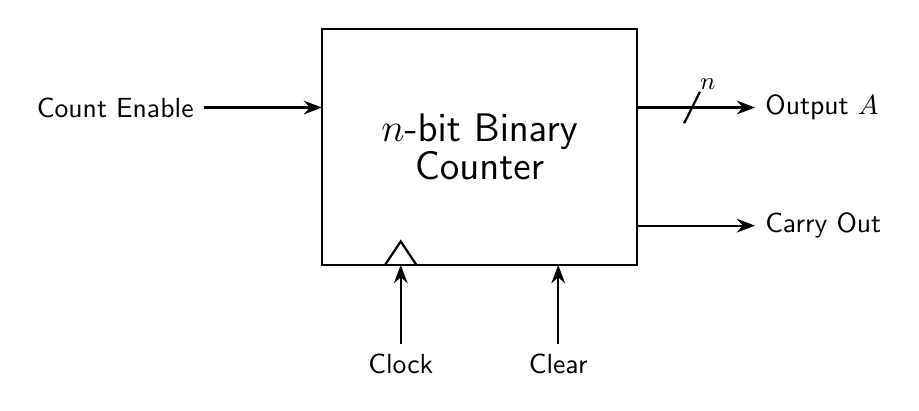
\begin{tikzpicture}[
    thick,
    >=Stealth,
    font=\sffamily
]

    % Counter Block
    \draw[fill=white] (0,0) rectangle (4,3);
    \node at (2,1.5) [align=center] {\Large $n$-bit Binary\\ \Large Counter};

    % Inputs
    % Count Enable
    \draw[<-] (0, 2) -- (-1.5, 2) node[left] {Count Enable};
    
    % Clock (with triangle indicator)
    \draw[<-] (1, 0) -- (1, -1) node[below] {Clock};
    \draw (0.8, 0) -- (1, 0.3) -- (1.2, 0);

    % Clear
    \draw[<-] (3, 0) -- (3, -1) node[below] {Clear};

    % Outputs
    % Counts (Bus)
    \draw[->] (4, 2) -- (5.5, 2) node[right] {Output $A$};
    % Bus slash
    \draw (4.6, 1.8) -- (4.8, 2.2);
    \node at (4.9, 2.3) {\small $n$};

    % Carry Out
    \draw[->] (4, 0.5) -- (5.5, 0.5) node[right] {Carry Out};

\end{tikzpicture}
\end{document}
